Data for our preliminary results were collected using Google Forms. The
prototype would issue information to the user to take an entry survey, guide
them through the features, and finish with an exit survey. The two surveys
contained the following questions:

\begin{center}
  \begin{tabular}{|l|p{0.6\linewidth}|}
    \hline
    \multicolumn{2}{|c|}{\Large \textbf{Entry Survey}}\\
    \hline
    \multirow{6}{*}{\textbf{Demographics}}
 & Name \\ \cline{2-2}
 & Age \\\cline{2-2}
 & Gender \\\cline{2-2}
 & Education \\\cline{2-2}
 & Major \\\cline{2-2}
 & Primary OS \\
    \hline
    \multirow{6}{*}{\textbf{Usability of Shell}}
 & I think the command line is easy to use. \\ \cline{2-2}
 & I think the command line is more usable than a GUI. \\ \cline{2-2}
 & I feel comfortable using the shell. \\ \cline{2-2}
 & I prefer command line tools to GUI tools.\\ \cline{2-2}
 & I think I would prefer the shell if I understood it better (or already
   do).\\ \cline{2-2}
 & I think the shell is easy to learn.\\
    \hline
    \multirow{4}{*}{\textbf{Efficiency}}
 & I use piping and redirection. \\ \cline{2-2}
 & I use control structures in the shell.\\ \cline{2-2}
 & I use wild cards in the shell.\\
    \hline
    \multirow{5}{*}{\textbf{Knowledge}}
 & When presented with a problem, I know the commands to use. \\ \cline{2-2}
 & I feel that learning how to use new commands is easy. \\ \cline{2-2}
 & I use a wide array of commands. \\ \cline{2-2}
 & I feel that I have sufficient knowledge of the shell for what I need. \\
    \hline
    \multirow{1}{*}{\textbf{Qualitative}} & Explain what tasks you commonly carry
                                            out on in the shell.\\
    \hline
  \end{tabular}
\end{center}

\begin{center}
  \begin{tabular}{|l|p{0.6\linewidth}|}
    \hline \multicolumn{2}{|c|}{\textbf{\Large Exit Survey}} \\ \hline
    \multirow{4}{*}{\textbf{Usability}}
    & This system would improve my usage of the shell. \\ \cline{2-2}
    & This system would help me solve problems in the shell. \\ \cline{2-2}
    & This system is more usable than a traditional shell. \\ \cline{2-2}
    & I find the interface of the system inviting and usable. \\
    \hline
    \multirow{3}{*}{\textbf{Educational Value}}
    & This system would teach me commands in a more effective way than the
      status quo. \\ \cline{2-2}
    & This system would help me perform automation that I would not make on my
      own.\\ \cline{2-2}
    & Using this system would improve my understanding of all shells.\\
    \hline
    \multirow{3}{*}{\textbf{Intention}}
    & I would prefer this to the normal shell experience. \\ \cline{2-2}
    & I would use this system in the future. \\ \cline{2-2}
    & I would suggest this system to others. \\
    \hline
    \multirow{2}{*}{\textbf{Qualitative Critique}}
    & What did you like most about the system?  \\ \cline{2-2}
    & What do you think needs the most improvements? \\
    \hline
  \end{tabular}
\end{center}
In between these surveys we presented a demo of our system.

\subsection{Data Analysis}
Data analysis was carried out using the Julia language, along with various
statistical tools. A cursory data analysis was also provided by Google Sheets,
allow a look at the results from each question.

The first thing we want to do is understand the demographics of our
survey. Primarily, and somewhat unsurprisingly, we had male CS majors. Linux was
the dominant operating system, but there was representation from other
systems. Our education levels were quite divers. This combination serves well to
test our target audience.

% TODO: Probably make subfigs for this data?
\begin{figure}[ht]
  \centering
  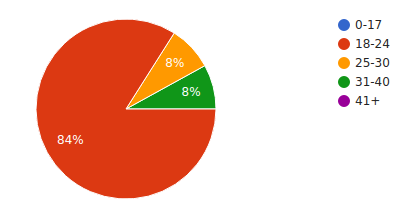
\includegraphics[width=0.8\linewidth]{figures/stats/age.png}
  \caption{\label{fig:age} Age demographics of survey base. }
\end{figure}

\begin{figure}[ht]
  \centering
  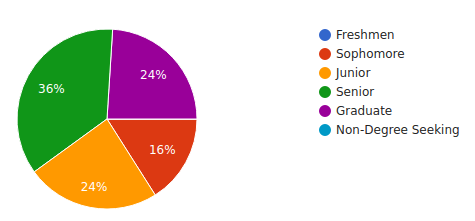
\includegraphics[width=0.8\linewidth]{figures/stats/edu.png}
  \caption{\label{fig:edu} Education demographics of survey base. }
\end{figure}

\begin{figure}[ht]
  \centering
  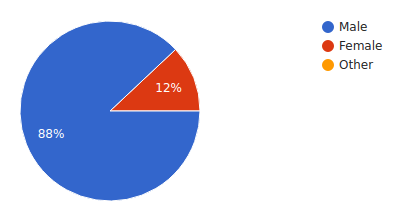
\includegraphics[width=0.8\linewidth]{figures/stats/gender.png}
  \caption{\label{fig:gender} Gender demographics of survey base. }
\end{figure}

\begin{figure}[ht]
  \centering
  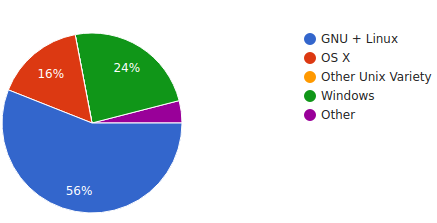
\includegraphics[width=0.8\linewidth]{figures/stats/os.png}
  \caption{\label{fig:OS} OS demographics of survey base. }
\end{figure}

We used the following Julia code to analyze the relative skill levels of our
users. Simply summing up the comfort level of all questions on the Entry survey,
we ranked users from Novice (0 experience) to Expert (39). Figure
\ref{fig:skill} shows a histogram representing user skill. You will notice that
the majority of our users are more experienced (self-reportedly). This does not
align with our target audience, however there was novice representation.
\begin{figure}[ht]
  \centering
  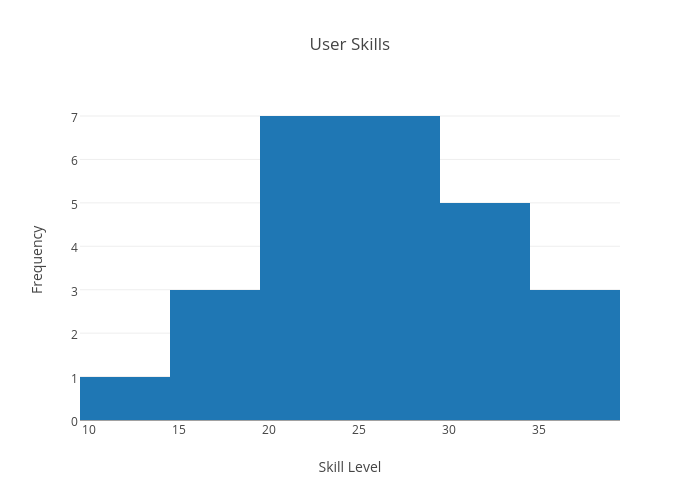
\includegraphics[width=0.8\linewidth]{figures/stats/user-skills.png}
  \caption{\label{fig:Skill} Histogram showing the relative skill levels of the
    user base. Note the larger right tail. }
\end{figure}


\subsection{Qualitative Analysis}
    8d. Describe the quantitative/qualitative analysis results with proper
    statistics test/grounded theory. You should also indicate whether or not the
    analysis result can support the hypotheses in Section 7.

%%% Local Variables:
%%% mode: latex
%%% TeX-master: "documentation"
%%% End:
